\documentclass[]{tufte-handout}
\usepackage{lmodern}
\usepackage{amssymb,amsmath}
\usepackage{ifxetex,ifluatex}
\usepackage{fixltx2e} % provides \textsubscript
\ifnum 0\ifxetex 1\fi\ifluatex 1\fi=0 % if pdftex
  \usepackage[T1]{fontenc}
  \usepackage[utf8]{inputenc}
\else % if luatex or xelatex
  \ifxetex
    \usepackage{mathspec}
    \usepackage{xltxtra,xunicode}
  \else
    \usepackage{fontspec}
  \fi
  \defaultfontfeatures{Mapping=tex-text,Scale=MatchLowercase}
  \newcommand{\euro}{€}
\fi
% use upquote if available, for straight quotes in verbatim environments
\IfFileExists{upquote.sty}{\usepackage{upquote}}{}
% use microtype if available
\IfFileExists{microtype.sty}{%
\usepackage{microtype}
\UseMicrotypeSet[protrusion]{basicmath} % disable protrusion for tt fonts
}{}
\usepackage{color}
\usepackage{fancyvrb}
\newcommand{\VerbBar}{|}
\newcommand{\VERB}{\Verb[commandchars=\\\{\}]}
\DefineVerbatimEnvironment{Highlighting}{Verbatim}{commandchars=\\\{\}}
% Add ',fontsize=\small' for more characters per line
\newenvironment{Shaded}{}{}
\newcommand{\KeywordTok}[1]{\textcolor[rgb]{0.00,0.44,0.13}{\textbf{{#1}}}}
\newcommand{\DataTypeTok}[1]{\textcolor[rgb]{0.56,0.13,0.00}{{#1}}}
\newcommand{\DecValTok}[1]{\textcolor[rgb]{0.25,0.63,0.44}{{#1}}}
\newcommand{\BaseNTok}[1]{\textcolor[rgb]{0.25,0.63,0.44}{{#1}}}
\newcommand{\FloatTok}[1]{\textcolor[rgb]{0.25,0.63,0.44}{{#1}}}
\newcommand{\CharTok}[1]{\textcolor[rgb]{0.25,0.44,0.63}{{#1}}}
\newcommand{\StringTok}[1]{\textcolor[rgb]{0.25,0.44,0.63}{{#1}}}
\newcommand{\CommentTok}[1]{\textcolor[rgb]{0.38,0.63,0.69}{\textit{{#1}}}}
\newcommand{\OtherTok}[1]{\textcolor[rgb]{0.00,0.44,0.13}{{#1}}}
\newcommand{\AlertTok}[1]{\textcolor[rgb]{1.00,0.00,0.00}{\textbf{{#1}}}}
\newcommand{\FunctionTok}[1]{\textcolor[rgb]{0.02,0.16,0.49}{{#1}}}
\newcommand{\RegionMarkerTok}[1]{{#1}}
\newcommand{\ErrorTok}[1]{\textcolor[rgb]{1.00,0.00,0.00}{\textbf{{#1}}}}
\newcommand{\NormalTok}[1]{{#1}}
\usepackage{longtable,booktabs}
\usepackage{graphicx}
\makeatletter
\def\maxwidth{\ifdim\Gin@nat@width>\linewidth\linewidth\else\Gin@nat@width\fi}
\def\maxheight{\ifdim\Gin@nat@height>\textheight\textheight\else\Gin@nat@height\fi}
\makeatother
% Scale images if necessary, so that they will not overflow the page
% margins by default, and it is still possible to overwrite the defaults
% using explicit options in \includegraphics[width, height, ...]{}
\setkeys{Gin}{width=\maxwidth,height=\maxheight,keepaspectratio}
\ifxetex
  \usepackage[setpagesize=false, % page size defined by xetex
              unicode=false, % unicode breaks when used with xetex
              xetex]{hyperref}
\else
  \usepackage[unicode=true]{hyperref}
\fi
\hypersetup{breaklinks=true,
            bookmarks=true,
            pdfauthor={Ben Bolker},
            pdftitle={introduction (week 1)},
            colorlinks=true,
            citecolor=blue,
            urlcolor=blue,
            linkcolor=magenta,
            pdfborder={0 0 0}}
\urlstyle{same}  % don't use monospace font for urls
\setlength{\parindent}{0pt}
\setlength{\parskip}{6pt plus 2pt minus 1pt}
\setlength{\emergencystretch}{3em}  % prevent overfull lines
\setcounter{secnumdepth}{0}

\title{introduction (week 1)}
\author{Ben Bolker}
\date{13:40 03 January 2015}

\begin{document}
\maketitle

\section{Introduction}\label{introduction}

\subsection{Administrative trivia}\label{administrative-trivia}

\begin{itemize}
\itemsep1pt\parskip0pt\parsep0pt
\item
  Instructor: Ben Bolker

  \begin{itemize}
  \itemsep1pt\parskip0pt\parsep0pt
  \item
    \texttt{bolker@mcmaster.ca}: please include \texttt{1mp3} in
    Subject:
  \item
    \texttt{http://www.math.mcmaster.ca/bolker}
  \item
    HH 314 (sometimes LSB 336); office hours TBA
  \end{itemize}
\item
  TA: Jake Szamosi
\item
  Grading:

  \begin{itemize}
  \itemsep1pt\parskip0pt\parsep0pt
  \item
    midterm 20\%
  \item
    final (take-home?) 30\%
  \item
    weekly assignments 30\%
  \item
    project 20\%
  \end{itemize}
\item
  Laptop policy
\item
  Course material on \href{https://github.com/bbolker/math1mp}{Github}
  and Avenue
\item
  Expectations of professor and students
\item
  Textbook (none); see
  \href{https://github.com/bbolker/math1mp/misc/resources.md}{resources}
\item
  Course content: reasonable balance among

  \begin{itemize}
  \itemsep1pt\parskip0pt\parsep0pt
  \item
    nitty-gritty practical programming instruction:
  \end{itemize}
\end{itemize}

\begin{quote}
\ldots{} I just sat down in front of a text editor, with nothing but
thoughts, and ended up with a program that did exactly what I wanted it
to a few hours later \ldots{}
(\href{http://www.ankitpanda.com/pythonicity/}{ankit panda})
\end{quote}

\begin{itemize}
\item
  \begin{itemize}
  \itemsep1pt\parskip0pt\parsep0pt
  \item
    conceptual foundations of computing/computer science
  \item
    context/culture of mathematical/scientific computing
  \item
    interesting applications
  \end{itemize}
\end{itemize}

\section{More interesting stuff}\label{more-interesting-stuff}

\subsection{Using computers in math and
science}\label{using-computers-in-math-and-science}

\begin{itemize}
\itemsep1pt\parskip0pt\parsep0pt
\item
  math users vs.~understanders vs.~developers
\item
  develop conjectures; draw pictures; write manuscripts
\item
  mathematical proof (e.g.
  \href{http://en.wikipedia.org/wiki/Four_color_theorem}{four-colo(u)r
  theorem} and
  \href{http://math.stackexchange.com/questions/1084230/what-are-some-theorems-that-currently-only-have-computer-assisted-proofs}{other
  examples}); computer algebra
\item
  applied math: cryptography, tomography, logistics, finance, fluid
  dynamics, \ldots{}
\item
  applied statistics: bioinformatics, Big Data/analytics, \ldots{}
\item
  discrete vs.~continuous
\end{itemize}

\subsection{Fun!}\label{fun}

\textbf{Hello, world}

\begin{Shaded}
\begin{Highlighting}[]
\DataTypeTok{print}\NormalTok{(}\StringTok{'hello, python world!'}\NormalTok{)}
\end{Highlighting}
\end{Shaded}

\begin{verbatim}
## hello, python world!
\end{verbatim}

Python as a fancy calculator:

\begin{Shaded}
\begin{Highlighting}[]
\DataTypeTok{print}\NormalTok{(}\DecValTok{62}\NormalTok{**}\DecValTok{2}\NormalTok{*}\DecValTok{27}\NormalTok{/}\DecValTok{5+3}\NormalTok{)}
\end{Highlighting}
\end{Shaded}

\begin{verbatim}
## 20760
\end{verbatim}

\begin{itemize}
\itemsep1pt\parskip0pt\parsep0pt
\item
  \emph{reference}:
  \href{https://docs.python.org/3/tutorial/introduction.html}{Python
  intro section 3.1.1}
\end{itemize}

\subsection{Interlude: about Python}\label{interlude-about-python}

\begin{itemize}
\itemsep1pt\parskip0pt\parsep0pt
\item
  \href{http://en.wikipedia.org/wiki/Scripting_language}{scripting};
  high-level; glue; general-purpose; flexible

  \begin{itemize}
  \itemsep1pt\parskip0pt\parsep0pt
  \item
    contrast: \emph{domain-specific} scripting languages (MATLAB, R,
    Mathematica, Maple)
  \item
    contrast: \emph{general-purpose} scripting languages (Perl, PHP)
  \item
    contrast: general-purpose \emph{compiled} languages (Java, C, C++)
    (``close to the metal'')
  \end{itemize}
\item
  relatively modern (1990s; Python 3, 2008)
\item
  currently the
  \href{http://www.tiobe.com/index.php/content/paperinfo/tpci/index.html}{8th
  most popular computer language} overall;
  \href{http://cacm.acm.org/blogs/blog-cacm/176450-python-is-now-the-most-popular-introductory-teaching-language-at-top-us-universities/fulltext}{most
  popular for teaching}
\item
  well suited to mathematical and scientific programming
  (\href{http://www.numpy.org}{NumPy};
  \href{http://www.scipy.org}{SciPy})
\item
  ex.: \href{http://www.sagemath.org}{Sage};
  \href{http://www.biopython.org}{BioPython}
\end{itemize}

\textbf{the Mandelbrot set}

Suppose we iterate \(z_{n+1}=z_{n}^2+c\), for some complex number \(c\),
starting with \(z_0=0\). The
\href{https://en.wikipedia.org/wiki/Mandelbrot_set}{Mandelbrot set} is
the set for which the iterations do \emph{not} go off to infinity.
(\emph{What happens for \(c=0\)? \(c=-1\)? \(c=i\)? \(c=1\)?})

We can iterate by hand \ldots{}

\begin{Shaded}
\begin{Highlighting}[]
\DataTypeTok{print}\NormalTok{(}\DataTypeTok{complex}\NormalTok{(}\DecValTok{0}\NormalTok{,}\FloatTok{0.65}\NormalTok{)**}\DecValTok{2}\NormalTok{+}\DataTypeTok{complex}\NormalTok{(}\DecValTok{0}\NormalTok{,}\FloatTok{0.65}\NormalTok{))}
\DataTypeTok{print}\NormalTok{((}\DataTypeTok{complex}\NormalTok{(}\DecValTok{0}\NormalTok{,}\FloatTok{0.65}\NormalTok{)**}\DecValTok{2}\NormalTok{+}\DataTypeTok{complex}\NormalTok{(}\DecValTok{0}\NormalTok{,}\FloatTok{0.65}\NormalTok{))**}\DecValTok{2}\NormalTok{+}\DataTypeTok{complex}\NormalTok{(}\DecValTok{0}\NormalTok{,}\FloatTok{0.65}\NormalTok{))}
\DataTypeTok{print}\NormalTok{(((}\DataTypeTok{complex}\NormalTok{(}\DecValTok{0}\NormalTok{,}\FloatTok{0.65}\NormalTok{)**}\DecValTok{2}\NormalTok{+}\DataTypeTok{complex}\NormalTok{(}\DecValTok{0}\NormalTok{,}\FloatTok{0.65}\NormalTok{))**}\DecValTok{2}\NormalTok{+}\DataTypeTok{complex}\NormalTok{(}\DecValTok{0}\NormalTok{,}\FloatTok{0.65}\NormalTok{))**}\DecValTok{2}\NormalTok{)+}\DataTypeTok{complex}\NormalTok{(}\DecValTok{0}\NormalTok{,}\FloatTok{0.65}\NormalTok{)}
\end{Highlighting}
\end{Shaded}

\begin{verbatim}
## (-0.4225+0.65j)
## (-0.24399375+0.10075j)
## (0.0493823875391+0.600835259375j)
\end{verbatim}

Use \textbf{assignments} to simplify \ldots{}

\begin{Shaded}
\begin{Highlighting}[]
\NormalTok{z0=}\DecValTok{0}
\NormalTok{c=}\DataTypeTok{complex}\NormalTok{(}\DecValTok{0}\NormalTok{,}\FloatTok{0.65}\NormalTok{)}
\NormalTok{z1=z0**}\DecValTok{2}\NormalTok{+c}
\NormalTok{z2=z1**}\DecValTok{2}\NormalTok{+c}
\NormalTok{z3=z2**}\DecValTok{2}\NormalTok{+c}
\DataTypeTok{print}\NormalTok{(}\DataTypeTok{abs}\NormalTok{(z3)<}\DecValTok{2}\NormalTok{)}
\end{Highlighting}
\end{Shaded}

\begin{verbatim}
## True
\end{verbatim}

The basic method for generating pretty pictures is:

\begin{itemize}
\itemsep1pt\parskip0pt\parsep0pt
\item
  for lots of different values of \(c\)

  \begin{itemize}
  \itemsep1pt\parskip0pt\parsep0pt
  \item
    set \(z_0=0\)
  \item
    keep calculating \(z_{n+1}=z_n^2+c\) until \(\textrm{mod}(z_{n+1})\)
    is greater than 2
  \item
    record the final value of \(n\)
  \end{itemize}
\item
  translate values of \(n\) into some colour scale and plot the results
\end{itemize}

Complex arithmetic is built into Python\\(\emph{What is
\((2+3i)^2\)=}\texttt{(complex(2,3))**2}?)

\href{../code/mandelbrot.py}{Mandelbrot set program}

\textbf{Note}:

\begin{itemize}
\itemsep1pt\parskip0pt\parsep0pt
\item
  easier to understand/modify than write from scratch
\item
  build on existing components (\emph{modules})
\end{itemize}

\subsection{Interfaces}\label{interfaces}

\begin{itemize}
\itemsep1pt\parskip0pt\parsep0pt
\item
  command line/console (PyCharm:
  \texttt{View/Tool Windows/Python Console})
\item
  programming editor
\item
  integrated development environment (IDE)
\item
  \textbf{not} MS Word! 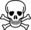
\includegraphics{pix/skullcross_tiny.png}
\end{itemize}

\textbf{Features}

\begin{itemize}
\item
  syntax highlighting
\item
  bracket-matching
\item
  hot-pasting
\item
  integrated help
\item
  integrated debugging tools
\item
  integrated project management tools
\item
  \textbf{most important}: maintain reproducibility; well-defined
  \textbf{workflows}
\end{itemize}

\section{Assignment}\label{assignment}

\begin{itemize}
\itemsep1pt\parskip0pt\parsep0pt
\item
  superficially simple

  \begin{itemize}
  \itemsep1pt\parskip0pt\parsep0pt
  \item
    \texttt{=} is the \textbf{assignment operator}
  \item
    \texttt{\textless{}variable\textgreater{}=\textless{}value\textgreater{}}
  \item
    variable names

    \begin{itemize}
    \itemsep1pt\parskip0pt\parsep0pt
    \item
      what is legal? (letters, numbers, underscores, start with a
      letter)
    \item
      what is customary?
      \href{https://www.python.org/dev/peps/pep-0008/\#id30}{convention}
      is \texttt{variables\_like\_this}
    \item
      what works well? \texttt{v} vs.
      \texttt{temporary\_variable\_for\_loop}
    \end{itemize}
  \end{itemize}
\item
  variables can be of different
  \href{https://docs.python.org/3/library/stdtypes.html}{\textbf{types}}

  \begin{itemize}
  \itemsep1pt\parskip0pt\parsep0pt
  \item
    built-in: integer (\texttt{int}), floating-point (\texttt{float}),
    complex, \textbf{Boolean} (\texttt{bool}: \texttt{True} or
    \texttt{False}),
  \item
    \emph{dynamic} typing
  \item
    (relatively) \emph{strong} typing

    \begin{itemize}
    \itemsep1pt\parskip0pt\parsep0pt
    \item
      try \texttt{print(type(x))} for different possibilities
      (\texttt{x=3}; \texttt{x=3.0}; \texttt{x="a"})
    \item
      \emph{what happens if you try \texttt{x=a}?}
    \item
      \textbf{don't be afraid to experiment!}
    \end{itemize}
  \end{itemize}
\end{itemize}

\begin{Shaded}
\begin{Highlighting}[]
\NormalTok{x=}\DecValTok{3}
\NormalTok{y=}\FloatTok{3.0}
\NormalTok{z=}\StringTok{"a"}
\NormalTok{q=}\DataTypeTok{complex}\NormalTok{(}\DecValTok{1}\NormalTok{,}\DecValTok{2}\NormalTok{)}
\DataTypeTok{type}\NormalTok{(x+y)  }\CommentTok{## mixed arithmetic}
\DataTypeTok{type}\NormalTok{(}\DataTypeTok{int}\NormalTok{(x+y))  }\CommentTok{## int(), float() convert explicitly}
\DataTypeTok{type}\NormalTok{(x+z)}
\DataTypeTok{type}\NormalTok{(q)}
\DataTypeTok{type}\NormalTok{(x+q)}
\DataTypeTok{type}\NormalTok{(}\OtherTok{True}\NormalTok{)}
\DataTypeTok{type}\NormalTok{(}\OtherTok{True}\DecValTok{+1}\NormalTok{) }\CommentTok{## WAT}
\end{Highlighting}
\end{Shaded}

\subsection{Comparisons and logical
expressions}\label{comparisons-and-logical-expressions}

\begin{itemize}
\itemsep1pt\parskip0pt\parsep0pt
\item
  comparison: (\texttt{==}, \texttt{!=})
\item
  inequalities: \texttt{\textgreater{}}, \texttt{\textless{}},
  \texttt{\textgreater{}=}, \texttt{\textless{}=},
\item
  basic logic: (\texttt{and}, \texttt{or}, \texttt{not})
\item
  remember your truth tables, e.g. \texttt{not(a and b)} equals
  \texttt{(not a) or (not b)}
\end{itemize}

\begin{Shaded}
\begin{Highlighting}[]
\NormalTok{a = }\OtherTok{True}\NormalTok{; b = }\OtherTok{False}\NormalTok{; c=}\DecValTok{1}\NormalTok{; d=}\DecValTok{0}
\NormalTok{a and b}
\NormalTok{not(a and not b)}
\NormalTok{a and not(b>c)}
\NormalTok{a==c  }\CommentTok{## careful!}
\NormalTok{not(d)}
\NormalTok{not(c)}
\end{Highlighting}
\end{Shaded}

\begin{itemize}
\itemsep1pt\parskip0pt\parsep0pt
\item
  \textbf{operator precedence}: same issue as
  \href{http://xkcd.com/992/}{order of operations in arithmetic};
  \texttt{not} has higher precedence than \texttt{and}, \texttt{or}.
  When in doubt use parentheses \ldots{}
\end{itemize}

\subsection{String operations}\label{string-operations}

\emph{reference}:
\href{https://docs.python.org/3/tutorial/introduction.html}{Python
intro} section 3.1.2

\begin{itemize}
\itemsep1pt\parskip0pt\parsep0pt
\item
  Less generally important, but fun
\item
  \texttt{+} concatenates
\item
  \texttt{*} replicates and concatenates
\item
  \texttt{in} searches for a substring
\end{itemize}

\begin{Shaded}
\begin{Highlighting}[]
\NormalTok{a = }\StringTok{"xyz"}
\NormalTok{b = }\StringTok{"abc"}
\NormalTok{a}\DecValTok{+1}  \CommentTok{## error}
\NormalTok{a+b}
\NormalTok{b*}\DecValTok{3}
\NormalTok{(a+}\StringTok{" "}\NormalTok{)*}\DecValTok{5}
\NormalTok{b in a}
\end{Highlighting}
\end{Shaded}

\subsection{Regular expressions}\label{regular-expressions}

Large topic -- somewhat more advanced than `basic programming', but
worth a digression.

What if we are looking for some number, but we don't know what number?

\begin{Shaded}
\begin{Highlighting}[]
\CharTok{import} \NormalTok{re}
\DataTypeTok{bool}\NormalTok{(re.search(}\StringTok{'[0-9]'}\NormalTok{, }\StringTok{'Plan 9'}\NormalTok{))}
\end{Highlighting}
\end{Shaded}

\begin{longtable}[c]{@{}cl@{}}
\toprule
\begin{minipage}[b]{0.17\columnwidth}\centering\strut
Pattern
\strut\end{minipage} &
\begin{minipage}[b]{0.59\columnwidth}\raggedright\strut
Description
\strut\end{minipage}\tabularnewline
\midrule
\endhead
\begin{minipage}[t]{0.17\columnwidth}\centering\strut
\texttt{\^{}}
\strut\end{minipage} &
\begin{minipage}[t]{0.59\columnwidth}\raggedright\strut
Beginning of line
\strut\end{minipage}\tabularnewline
\begin{minipage}[t]{0.17\columnwidth}\centering\strut
\texttt{\$}
\strut\end{minipage} &
\begin{minipage}[t]{0.59\columnwidth}\raggedright\strut
End of line
\strut\end{minipage}\tabularnewline
\begin{minipage}[t]{0.17\columnwidth}\centering\strut
\texttt{.}
\strut\end{minipage} &
\begin{minipage}[t]{0.59\columnwidth}\raggedright\strut
Any single character except newline
\strut\end{minipage}\tabularnewline
\begin{minipage}[t]{0.17\columnwidth}\centering\strut
\texttt{{[}...{]}}
\strut\end{minipage} &
\begin{minipage}[t]{0.59\columnwidth}\raggedright\strut
Any single character in brackets
\strut\end{minipage}\tabularnewline
\begin{minipage}[t]{0.17\columnwidth}\centering\strut
\texttt{{[}\^{}...{]}}
\strut\end{minipage} &
\begin{minipage}[t]{0.59\columnwidth}\raggedright\strut
Any single character \textbf{not} in brackets
\strut\end{minipage}\tabularnewline
\begin{minipage}[t]{0.17\columnwidth}\centering\strut
\texttt{re*}
\strut\end{minipage} &
\begin{minipage}[t]{0.59\columnwidth}\raggedright\strut
0 or more occurrences of preceding expression
\strut\end{minipage}\tabularnewline
\begin{minipage}[t]{0.17\columnwidth}\centering\strut
\texttt{re+}
\strut\end{minipage} &
\begin{minipage}[t]{0.59\columnwidth}\raggedright\strut
1 or more occurrence of preceding expression
\strut\end{minipage}\tabularnewline
\begin{minipage}[t]{0.17\columnwidth}\centering\strut
\texttt{re?}
\strut\end{minipage} &
\begin{minipage}[t]{0.59\columnwidth}\raggedright\strut
0 or 1 occurrence of preceding expression
\strut\end{minipage}\tabularnewline
\begin{minipage}[t]{0.17\columnwidth}\centering\strut
\texttt{re1\textbar{}re2}
\strut\end{minipage} &
\begin{minipage}[t]{0.59\columnwidth}\raggedright\strut
match \texttt{re1} or \texttt{re2}
\strut\end{minipage}\tabularnewline
\begin{minipage}[t]{0.17\columnwidth}\centering\strut
\texttt{()}
\strut\end{minipage} &
\begin{minipage}[t]{0.59\columnwidth}\raggedright\strut
grouping
\strut\end{minipage}\tabularnewline
\bottomrule
\end{longtable}

\begin{itemize}
\itemsep1pt\parskip0pt\parsep0pt
\item
  How would you test whether a string contains a numeric value at the
  end (e.g. ``Plan 99'')?
\item
  What if the string might contain a comma (e.g. ``Plan 99,478'')?
\item
  What if you're looking for the abbreviations of rooms in Hamilton Hall
  (my office is HH314)?
\item
  \ldots{} rooms in LSB \emph{or} HH?
\end{itemize}

\section{Lists and indexing}\label{lists-and-indexing}

\emph{reference}:
\href{https://docs.python.org/3/tutorial/introduction.html}{Python
intro} section 3.1.3

\subsection{Lists}\label{lists}

\begin{itemize}
\item
  Use square brackets \texttt{{[}{]}} to set up a \textbf{list}
\item
  Lists can contain anything but usually homogeneous
\item
  Put other variables into lists
\item
  Put lists into lists!
\item
  \texttt{range()} makes a \textbf{range} but you can turn it into a
  list with \texttt{list()}
\item
  \emph{Make a list that runs from 101 to 200}
\item
  \emph{Make a list that \ldots{} }
\end{itemize}

\subsection{Indexing and slicing}\label{indexing-and-slicing}

\textbf{Indexing}

\begin{itemize}
\itemsep1pt\parskip0pt\parsep0pt
\item
  Extracting elements is called \textbf{indexing} a list
\item
  Indexing \href{http://xkcd.com/163/}{starts from zero}
\item
  Negative indices count backward from the end of the string\\(-1 is the
  last element)
\item
  Indexing a non-existent element gives an error
\end{itemize}

\begin{figure}[htbp]
\centering
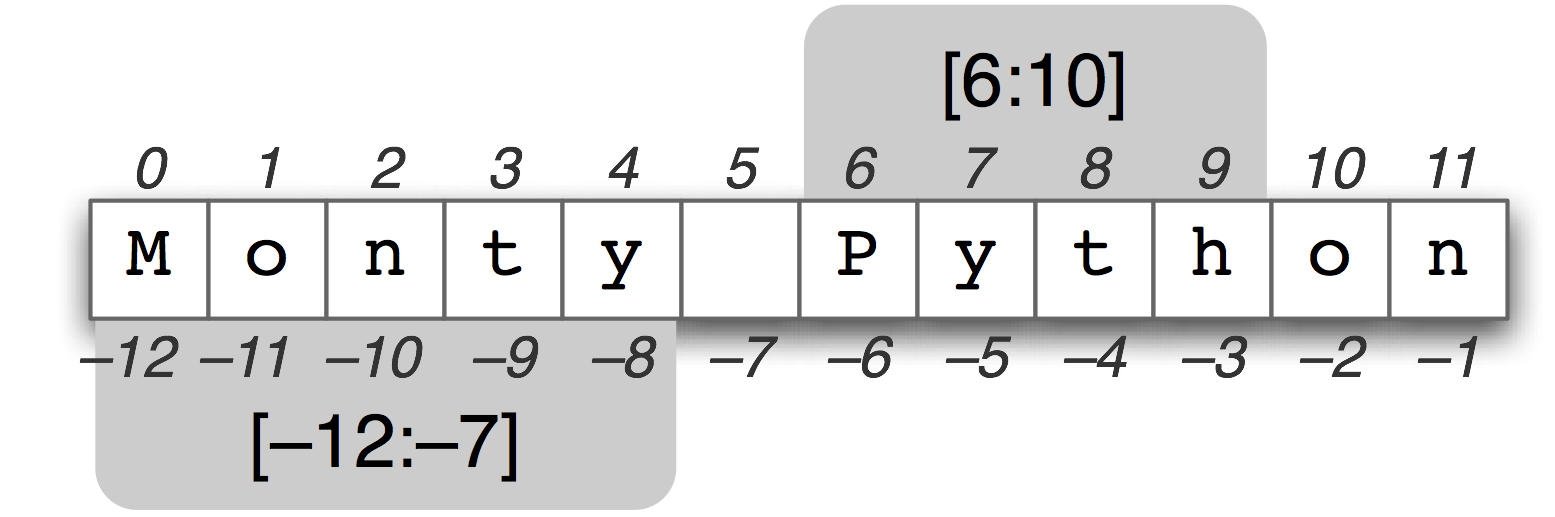
\includegraphics{pix/string-slicing.png}
\caption{slicing}
\end{figure}

\textbf{Slicing}

\begin{itemize}
\itemsep1pt\parskip0pt\parsep0pt
\item
  Extracting sets of elements is called
  \href{http://stackoverflow.com/questions/509211/explain-pythons-slice-notation}{\textbf{slicing}}
\item
  Slicing non-existent element(s) gives a truncated result
\item
  Slicing specifies \emph{start}, \emph{end}, \emph{step} (or
  ``stride'')
\item
  Leaving out a bit goes from the beginning/to the end
\item
  Slicing works on strings too!
\end{itemize}

\begin{Shaded}
\begin{Highlighting}[]
\NormalTok{x[:]        }\CommentTok{# everything}
\NormalTok{x[a:b]      }\CommentTok{# element a (zero-indexed) to b-1}
\NormalTok{x[a:]       }\CommentTok{# a to end}
\NormalTok{x[:b]       }\CommentTok{# beginning to b}
\NormalTok{x[a:b:n]    }\CommentTok{# from a to b-1 in steps of n}
\end{Highlighting}
\end{Shaded}

\begin{itemize}
\itemsep1pt\parskip0pt\parsep0pt
\item
  generate list of odd numbers from 3 to 15
\item
  reverse a string?
\end{itemize}

\textbf{Other list operations}

\begin{itemize}
\itemsep1pt\parskip0pt\parsep0pt
\item
  Lots of things you can do with lists!
\item
  Distinguish between \emph{copying} lists and modifying them in-place
\item
  Distinguish between \emph{functions} and \emph{methods}
  \texttt{foo(x)} vs. \texttt{x.foo()}

  \begin{itemize}
  \itemsep1pt\parskip0pt\parsep0pt
  \item
    appending:
  \item
    list
    \href{http://www.linuxtopia.org/online_books/programming_books/python_programming/python_ch14s07.html}{\emph{methods}}
  \item
    appending and extending:
  \end{itemize}
\end{itemize}

\begin{Shaded}
\begin{Highlighting}[]
\NormalTok{x = [}\DecValTok{1}\NormalTok{,}\DecValTok{2}\NormalTok{,}\DecValTok{3}\NormalTok{]}
\NormalTok{y = [}\DecValTok{4}\NormalTok{,}\DecValTok{5}\NormalTok{]}
\NormalTok{x.append(y)}
\DataTypeTok{print}\NormalTok{(x)}
\end{Highlighting}
\end{Shaded}

\begin{verbatim}
## [1, 2, 3, [4, 5]]
\end{verbatim}

\begin{Shaded}
\begin{Highlighting}[]
\NormalTok{x = [}\DecValTok{1}\NormalTok{,}\DecValTok{2}\NormalTok{,}\DecValTok{3}\NormalTok{] }\CommentTok{# reset x}
\NormalTok{y = [}\DecValTok{4}\NormalTok{,}\DecValTok{5}\NormalTok{]}
\NormalTok{x.extend(y)}
\DataTypeTok{print}\NormalTok{(x)}
\end{Highlighting}
\end{Shaded}

\begin{verbatim}
## [1, 2, 3, 4, 5]
\end{verbatim}

Can use \texttt{+} as a shortcut for extending:

\begin{Shaded}
\begin{Highlighting}[]
\NormalTok{x = [}\DecValTok{1}\NormalTok{,}\DecValTok{2}\NormalTok{,}\DecValTok{3}\NormalTok{]}
\NormalTok{y = [}\DecValTok{4}\NormalTok{,}\DecValTok{5}\NormalTok{]}
\NormalTok{z = x+y}
\DataTypeTok{print}\NormalTok{(z)}
\end{Highlighting}
\end{Shaded}

\begin{verbatim}
## [1, 2, 3, 4, 5]
\end{verbatim}

\begin{itemize}
\itemsep1pt\parskip0pt\parsep0pt
\item
  \texttt{x.insert(position,value)}: inserts
\item
  \texttt{x.remove(value)}:
\item
  \texttt{x.pop(position)} (or \texttt{del x{[}position{]}} or
  \texttt{x{[}position{]}={[}{]}})
\item
  \texttt{x.reverse()} (or \texttt{x{[}::-1{]}})
\item
  \texttt{x.sort()}: what it says
\item
  \texttt{x.count(value)}: number of occurrences of \texttt{value}
\item
  \texttt{x.index(value)}: first occurrence of \texttt{value}
\item
  \texttt{value in x}: does \texttt{value} occur in \texttt{x}? (or
  \texttt{logical(x.count(value)==0)})
\item
  \texttt{len(x)}: length
\end{itemize}

\textbf{Note}:
\href{http://blog.startifact.com/posts/older/what-is-pythonic.html}{pythonicity}
vs.
\href{http://en.wikipedia.org/wiki/There\%27s_more_than_one_way_to_do_it}{TMTOWTDI}

\end{document}
